\chapter{Background Knowledge}
\label{ch:background}
To understand the chapters ahead and ease the reader into this work, here are defined all the required notions on which DevArtist and its evaluation rely on. In addition, this chapter offers the necessary terminology and a place to reference later in the thesis. For obvious reasons, all the information provided here will be focused on Android but, where possible, attempts to provide the general idea are made.

\section{Android Architecture}
Android can be seen as a heavily customized Linux distribution, where Andy Rubin and his team, the original developers of Android, implemented a set of features and a UI framework with the goal to target mobile devices. Sharing the kernel with other distributions makes it easier for hardware companies to write drivers and enables Android to use a multitude of already existing C/C++ libraries which have been developed and tested through the years. In addition, the OS also abstracts those libraries and allows application developers to make use of them through a Java API: the Android SDK. A simplified version of the Android software stack is reported in Fig: \ref{fig:androidstack}, a full version of its documentation is available in \cite{and_doc_stack}.

\begin{figure}
	\centering
	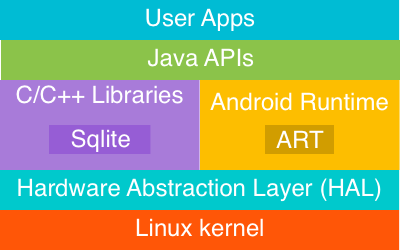
\includegraphics[scale=0.8]{img/android_stack.png}
	\caption{Android Platform Overview\cite{artist}}
	\label{fig:androidstack}
\end{figure}

\section{Android's Application Package}
Any Android developer can develop apps through the Android SDK provided by Google. The main language is Java but it's also possible to use the Android NDK and develop in C/C++, even though it's not suggested. At the moment of writing also Kotlin, a language that compiles to JVM byte-code, is officially supported and it is gaining momentum. Moreover, when an app is ready, its code gets compiled through the \texttt{javac}  compiler and \texttt{dx} tool, which transforms all the \emph{.class} files into one or more\emph{.dex} files, which are compatible with the Dalvik Virtual Machine (DVM). Successively, the produced byte-code is compressed together with other files, such as the Manifest and developer signature, forming the Android's application package (APK).

\section{Android Internals}
The following subsections offer information about one service and one API, which are provided by the OS and are important because mentioned throughout this thesis.

\subsection{The Logcat}
On Android, there is no standard output and every call to the \texttt{System.out.println} (depending on the implementation by the device manufacturer) gets redirected by the OS to the default logging system. This system can be used by developers through the \texttt{Log} class and it provides three main levels of messages: ERROR, WARN and INFO. Moreover, all the log messages produced by both the OS and developers can be analyzed through the Logcat program, which is shipped within the Android Debug Bridge (ADB, a collection of development programs for Android) and integrated in both Android Studio and Eclipse.

\subsection{Public Components}
\label{sc:exportedcomponents}
Among the primary building blocks of the Android ecosystem, there are re-usable components: specific parts of an application's code which can be used also by other applications installed on a device. The goal of such a system is to provide developers a way to make use of  data and computation of other apps without the need to manually gather the information or code an extra functionality. An example of this behavior can be found every time an application, such as Evernote, needs to save an appointment: it can open the default calendar application and let the UI of this latter application handle the appointment creation and sync with a server. Another example might be a medical application which lists all the checks that a patient needs to attend to: in this case, it can ask the calendar application to provide all the appointments with the flag \enquote{medical} or \enquote{Dr.} and display them without actually managing the data. The system also prevents that different application alienate the user with different UIs for the same task, providing better consistency across the platform. However, this components might be dangerous from a privacy standpoint, due to the fact that, through them, applications which do not have permissions to view sensitive information, instead manage to gather access to it.


\section{Application Analysis}
There are many kinds of automated analysis, which can be performed on programs and, consequently, on mobile applications. The sub-genre, on which we focus, is letting another program perform an inquiry on the security of an arbitrary application. Moreover, this kind of examination branches in two separate directions, depending at which level of the software is executed, specifically: static analysis works on the source code or byte-code level of an application, whilst dynamic analysis is computed at runtime. There are advantages and disadvantages in both of them, although our system, as many others, combines them in order to achieve better accuracy.
It would be easy to think that instrumenting Android applications could be simple enough and that any tool developed for GNU/Linux up to now could be used, as also done by Min Zheng et al in DroidTrace\cite{droidtrace}, where they leveraged \emph{ptrace} to perform dynamic analysis. However, this is not the case due to the fact that this technique allows to perform the analysis only on the lowest part of the Android software stack, precisely the kernel system calls, leaving open the analysis at the level of Java APIs. 

\section{Application Instrumentation}
Instrumenting an application fundamentally means extending static or dynamic analysis to the point of changing or extending its behavior. In fact, popular uses of instrumentation are: code-tracing, profiling and even debugging. Instrumentation also is sub-divided in two branches and its named source instrumentation the one which operates at the source code or byte-code level, while the name binary instrumentation is used whenever the changes apply at the executable level. The most common way to instrument applications is via hooking specific parts of the code and then call another one, implemented separately, whenever that point is reached. This technique, used jointly with Inline Reference Monitoring (IRM)\cite{irm}, has been modified and employed on Android by quite a few researchers. In fact, as shown by AspectDroid\cite{AspectDroid}, CHEX\cite{chex} and others, this technique is still valid and allows to hook Android application's byte-code. However, on this OS, this approach also requires re-packaging, which consists in extracting all the code and resources from one apk to copy them into a new one with the changes needed to hook. Moreover, for security reasons, the Android system requires each apk to be signed and, since the original signature is known only to the app's developer, the approach must include another signature. Signing with a different key breaks application updates for users though, since the Play Store uses it to verify apks. Therefore, this thesis aims to keep these possibilities for the user and base its novelty on the new approach provided by the Android Runtime.


\section{Android Runtime}
The Android Runtime (ART) introduced ahead-of-time compilation (AOT) since Android 4.4 and made it the default on Android 5, definitely replacing  the DVM. This change did not only improve app performance, but also required a shorter app installation time. However, changing the way applications are compiled and executed could have meant significant losses in the amount of already published apps on the store because of incompatibility with the new system. Therefore, Google's engineers maintained the compatibility with the DEX file format by using an on-device compiler called \textbf{dex2oat}, which takes the Dalvik code (dex code) and transpiles it to native machine code. Due to the nature of Android, this compiler is greatly modularized and it is capable of generating native code for a multitude of architectures, such as: mips, mips64, x86, x64 arm and arm64. In particular, dex2oat defines three backends: \emph{Quick}, \emph{Portable} and \emph{Optimizing}, all of them specify a different behavior regarding how the dex code is handled. However, since the first is strictly derived from the DVM and the future of the second is uncertain\cite{artist}, in this thesis we focus more on the latter. 

\subsection{Optimizing Backend}
This backend option became the default for app compilation since the release of Android 6 Marshmallow, dropping the \emph{Quick} one almost completely, which is now only used to compile Android's boot image. The main reason for this change was that \emph{Optimizing} allowed state-of-the-art code optimization techniques such as the removal of: dead code, redundant bound check or even duplicate code. In particular, this backend defines a structure for developers to create optimization steps that work on the Intermediate Representation (IR) of the dex code contained in the APK file.

\subsubsection{Intermediate Representation}
ART's AOT compilation, as many other compilers, uses an Intermediate Representation (IR) before transforming dex code to machine code. In fact, the main role of dex2oat can be summarized as creating the IR from the dex code and then performing optimization steps on it. Moreover, the IR of a program can be seen as an oriented graph, where every instruction scanned from the beginning of the dex code represents a node. This particular form of this graph is called Control Flow Graph (CFG) because it maps every flow of the code, showing not only where it branches but also why. Specifically to the IR used by dex2oat, the instructions are reduced to single static assignment form (SSA), which is ensuring that every variable is assigned exactly once and they can be represented as a string having the following structure:
\begin{figure}[H]
\centering
\begin{BVerbatim}
instruction_id: instruction_type:method_name(inputs)[uses]
\end{BVerbatim}
\end{figure}
where the id is given by the compiler, the types are either: ParamValue (a parameter passed to a function), basic mathematical operations (add, xor, and, etc...) or the type of method which is invoked. However, there are many more types of instruction which this work does not analyze and they can be found in \cite{artist}. Furthermore, \emph{inputs} is a comma separated list of all the arguments that need to be passed into the method, whilst the \emph{uses} are also a comma separated list of all the other instructions, where that method is then used later in the code. Table \ref{tab:exampleAdd} offers an example of conversion from Java code to the IR.\newline

\begin{table}[h!]
  \centering
  \begin{tabular}{|c|}
  	\hline
	\begin{lstlisting}[language=Java]
	public int getRandomNumber(long seed){
		Random rnd = new Random(seed);
		return rnd.nextInt();
	}
	\end{lstlisting}\\
	\hline
	\begin{lstlisting}[language={[x86masm]Assembler}]
		getRandomNumber: Basic block 0
		0: ParamValue(this)
		1: ParamValue(Long)[3]
		2: newInstance:java.util.Random()[3]
		3: InvokeStaticOrDirect:java.util.Random<init>(1)[3]
		4: NullCheck(2)[5]
		5: InvokeVirtual:java.util.Random.nextInt(4)[6]
		6: Return(5)
	\end{lstlisting} \\
	\hline
  \end{tabular}
    \caption{Java code on the upper side, IR representation on the lower one}
	\label{tab:exampleAdd}
\end{table}

\subsection{The Special Case of NullCheck}
In order to avoid accessing null objects at runtime and throw a \texttt{NullpointerException}, the compiler inserts a special instruction before every method of an object instance gets called, which has type: \texttt{NullCheck}. As it can be also seen in Table \ref{tab:exampleAdd}, this instruction always has as it's first input a reference to instruction which contains the instantiation of the object upon the null check has to be computed upon. This property will come handy to compute backward slicing later in this work.


\section{Program Slicing}
An entire branch of Computer Science is dedicated to the field of Information Flow Control (IFC), which studies how data is passed and transformed by processes. In particular, especially in the security field, it is important to track the mutations of variables, to prevent data leaks and other privacy issues. Therefore, to achieve this goal, Reps and Yung introduce in \cite{slicing} the concept of program slicing and they define what is the \emph{Backward} and \emph{Forward} slice of a line of code, abbreviated in BS(x) and FS(x), but also, they prove formally that the BS(x) contains all the operations which influence a line of code x. In fact, the BS(x) is the collection of all the previous lines of code that cause a change to x, whilst FS(x) is the collection of all the lines of code that follows x, which change when x does. Moreover, inside the BS(x) we can define a Source (So), which is the line where the tracked data is first defined, and a Sink (Si), which is the last usage of that data. Table \ref{tab:slicing} shows an example of slicing where the source is line 2 and sink is line 5, please mind that a sink can also be a return operation and not only an output operation. However, although the example shows slicing on Java code, slicing is the core of the optimizations steps performed on  IR by the Optimization backend and, consequently, Artist.    

\lstset{numbers=none}
\begin{table}[h!]
  \centering
  \begin{tabular}{|c|c|}
  	\hline
	\begin{lstlisting}[language=Java]
	public void Print10Bar(int n){
		int x = 10;
		bar(x+n);
		x++;
		System.out.println(x);
	}
	\end{lstlisting} &
	\begin{lstlisting}[language=Java]
		int x = 10;
		x++;
		System.out.println(x);
	\end{lstlisting} \\
	\hline
  \end{tabular}
    \caption{Java code on the left side, BS(5) on the right}
	\label{tab:slicing}
\end{table}


\section{Artist and ArtistGUI}
ARTist is a new Android instrumentation framework for security researchers and developers which stands on top of dex2oat's optimizing backend. It is composed of a static and a dynamic component: the first one is able to instrument the application at compile time, whilst the other is a library merged into the app. This method not only allows for better instrumentation but has serious advantages for the user, who can keep updating the application as they used to.

\subsection{Artist}
\label{sec:artist}
ART Optimizing backend implements a few optimization steps, which already work on the IR graph. Hence, the developers of \emph{ARTist} implemented it as a new optimization step, which is able to compute CRUD\footnote{Acronym for : Create, Read, Update, Delete} operations upon the IR, thus achieving static analysis and source instrumentation. Moreover, it enables third-party developers to hook the right instruction target(s) by implementing a visitor pattern on the IR graph, and then, it exposes helper methods which can replace, modify, move or even delete the chosen instruction(s). In this way, when the compilation actually happens, the resulting native code reflects the modified IR graph (IR*) and not the original one, thus allowing the change of behavior in the app. Figure \ref{fig:optbackend} provides a visual representation of the work-flow inside the newly changed Optimizing backend of dex2oat and helps in creating a mental map of the steps involved in the process.

\begin{figure}[H]
	\centering
	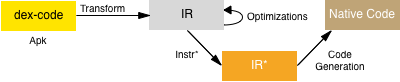
\includegraphics{img/dex2oat.png}
	\caption{The optimizing backend with Artist}
	\label{fig:optbackend}
\end{figure}

\subsection{ArtistGUI}
The dynamic analysis is provided by an Android app called ArtistGUI, which includes the dex2oat binary and enables the end-user to compile apps with it. Instead of statically linking the compiler, this app uses the \texttt{LD\_LIBRARY\_PATH} directive to ensure that all the libraries needed by dex2oat are loaded. Furthermore, the app shows a list of already installed apps and, when one is tapped on, it performs two main functions: first it merges an auxiliary library into the app and then it re-compiles the chosen app with its own dex2oat. The afore-mentioned library is also produced by the developer that creates the Artist module and it is often used both to perform the analysis of the app at runtime but also to aid the insertion of new instructions in the IR at compile level. In fact, since creating new code on the Artist side is hard due to its representation, developers can create this code in Java within the library and then insert them at the compiler level whenever they need by referencing it.

\begin{figure}[H]
	\centering
	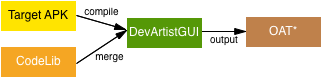
\includegraphics{img/devartistgui.png}
	\caption{The work-flow of ArtistGUI}
	\label{fig:installprocess}
\end{figure}

\section{Automated Testing}
Proving the need and the soundness of this work would have required too much time if executed manually, due to the fact that it had to be tested on real apps. Therefore, layers of automated testing has been set up, not only to download applications from the Google Play Store but also to instrument, check their behavior and automatically generate a full report, which can be manually analyzed to extract important information.

\subsection{Monkey Troop}
The developers of \emph{Artist} also provide \emph{Monkey Troop}, a python tool which can automatically test an \emph{Artist} module. This system is capable of installing applications, run them, tap on the screen as an user would do and instrument them with a specified module. It also generates a report, with the full Logcat (Android's standard output log) for each application. Unfortunately, the tool comes with little documentation, which is available with the code on Github \cite{monkeytroop}. However, the steps to use Monkey Troop are limited to defining a list of links to apps on the Play Store and creating a set of commands, which the system has to execute on a target device to successfully test the module. The device must already have the front-end of the module (ArtistGUI) installed and the tool automatically uses it to instrument every application on the above mentioned list.

\begin{figure}[H]
	\centering
	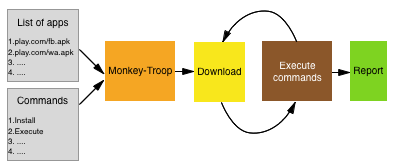
\includegraphics{img/monkey_troop.png}
	\caption{Monkey Troop Overview}
	\label{fig:monkeyoverview}
\end{figure}

